\documentclass[10pt,twocolumn,letterpaper]{article}

\usepackage{cvpr}
\usepackage{times}
\usepackage{epsfig}
\usepackage{graphicx}
\usepackage{amsmath}
\usepackage{amssymb}
\usepackage{siunitx}
\usepackage{textcomp}
\usepackage{setspace}
\doublespacing
% Include other packages here, before hyperref.

% If you comment hyperref and then uncomment it, you should delete
% egpaper.aux before re-running latex.  (Or just hit 'q' on the first latex
% run, let it finish, and you should be clear).
\usepackage[pagebackref=true,breaklinks=true,letterpaper=true,colorlinks,bookmarks=false]{hyperref}
% \cvprfinalcopy % *** Uncomment this line for the final submission

\def\cvprPaperID{****} % *** Enter the CVPR Paper ID here
\def\httilde{\mbox{\tt\raisebox{-.5ex}{\symbol{126}}}}

% Pages are numbered in submission mode, and unnumbered in camera-ready
\ifcvprfinal\pagestyle{empty}\fi
\begin{document}

%%%%%%%%% TITLE
\title{Layerd Optical Flow Estimation using Soft-masks Module in Deep Neural Network}

\author{First Author\\
Institution1\\
Institution1 address\\
{\tt\small firstauthor@i1.org}
% For a paper whose authors are all at the same institution,
% omit the following lines up until the closing ``}''.
% Additional authors and addresses can be added with ``\and'',
% just like the second author.
% To save space, use either the email address or home page, not both
\and
Second Author\\
Institution2\\
First line of institution2 address\\
{\tt\small secondauthor@i2.org}
}

\maketitle
%\thispagestyle{empty}

%%%%%%%%% ABSTRACT
\begin{abstract}
Layered representation to motion estimation has long been seen as promising and efficient, since spatial smoothness is separated from the modeling of discontinuities and occlusions. In this paper, we learn to estimation optical flow by combining layered motion representation and deep learning. Instead of pre-segmenting image to layers, the proposed approach will automatically generation layered representation of optical flow using the proposed soft-masks module. The essential parts of the soft-masks module are a maxout and a fuse operation, which enable a disjoint layered representation of optical flows and more accurate flow estimation using a quadratic function in terms of input features in output layer. The proposed soft-masks module can simply work as an add-on to replace flow output layer of existing optical flow estimation networks. In evaluation, we use FlowNet as our base net to add the soft-masks module. The resulting networks are tested on three well known benchmark with both supervised and unsupervised flow estimation tasks. Empirical results show that the proposed network achieve better results with respect to the original FlowNet. 
\end{abstract}

%%%%%%%%% BODY TEXT
\section{Introduction}
Optical flow estimation has long been an important thus challenging problem in computer vision research. We have observed a steady progress by improving performance on increasingly challenging benchmarks. The original formulation of optical flow estimation was introduced by Horn and Schunck in~\cite{horn1981determining}. The formulation resemble a data term which assume consistent image property with a spatial term which regularizes smoothness of the flow. Various of successful works are derived from this initial formulation by tweaking and fine tuning ingredients of flow estimation. 

Layered models of optical flow is one of these successful techniques, which offer an easy performance boost for optical flow estimation~\cite{wang1994representing}\cite{341161}\cite{darrell1995cooperative}. Disjointly splitting the optical flow into layers enable an easier modeling of optical flow in each layer. Such representation is especially helpful for small object motion estimation. Because many optical flow estimation techniques utilize a general bias for motion detected in a large area, which can easily ignored motions brought by small size objects. Layered representation will also improve flow computation on boundaries of flow field by handling the smoothness constraint separately in each layer.

FlowNet by Dosovitskiy~\cite{7410673} is the first work to use a deep neural network to end-to-end learn optical flow. The concept of training FlowNet was completely disjoint from established formula used by all previous approaches. Since many techniques used by traditional optical flow estimation are demonstrated to be truly helpful when addressing the problem of flow estimation.  Some deep learning based approaches later tried to bridge the gap between traditional approaches and deep learning based approaches by using the best from both side. Such as in~\cite{Ranjan_2017_CVPR}, a pyramid representation of flows associated with flow computation using residual flows is used to address large flow displacement problem. Several approaches~\cite{ren2017unsupervised}\cite{ahmadi2016unsupervised}\cite{DBLP:journals/corr/YuHD16} investigate basic principles of flow estimation and proposed to directly follow these principles by training networks unsupervisely.   

This paper combines the idea of using layered optical flow representation with deep neural network structure. Unlike previous approaches~\cite{yang2015dense}\cite{black1996estimating}\cite{ju1996skin}, where layered representation has to be generated separately. The layered representation in the proposed approach is inferred internally and automatically during training of neural networks. To enable such property, we introduce the soft-masks module in this work. Soft-masks module is a small network structure with simple but neat design which split optical flow to layers using disjoint masks of real value. This is where the name 'soft' comes from. Soft-masks module can offer a more accurate flow estimation due to its two unique characteristics. The first is ability to represent estimated flow using disjoint layers, which results in a more focused and simpler flow estimation for each layer. Second, compared with linear flow output in FlowNet, the flow estimated using soft-masks module is a quadratic form in terms of input features, which provide the soft-masks module a better computational power to fit more complicated optical flow cases. The idea of using soft-masks module is similar to the maxout networks proposed by Goodfellow~\cite{Goodfellow:2013:MN:3042817.3043084}, where the output of a neuron is the max of a set of inputs. The proposed soft-masks module is an extension of maxout operation in 2D case, where maxout operation is carried out through channels of input feature maps. Instead of keeping max value only, we zero-out non-max values and use these values as mask-out region when masks are fused with layered optical flows.

The soft-masks module can be simply used on FlowNet by replacing the output layer of the network with the soft-masks module. We are also investigating the eligibility of using soft-masks module for other per-pixel prediction tasks such as semantic segmentation~\cite{long2015fully}, single image depth estimation~\cite{eigen2014depth}, since these tasks can enjoy the same benefit brought by soft-masks module.

We do not claim to achieve state of the art performance by using FlowNet with the proposed soft-masks module. We emphasize on showing an easy performance boost can be obtained for FlowNet by using the proposed module. We also show in evaluation part that, both supervised and unsupervised flow estimation methods are expected to get improved by using the soft-masks module.

\subsection{Related Work}
Our work effectively combines ideas of using layered representation in classical optical flow approaches and recent deep learning approaches. Our literature review thus focuses on the work most relevant to this.
\newline
\newline
\noindent \textbf{Layered approaches.}
Layered approaches to motion estimation have long been demonstrated as elegant and effective, since spatial smoothness is separated from the modeling of discontinuities and occlusions. The pioneer work of Darrell and Pentland~\cite{darrell1991robust}\cite{darrell1995cooperative} provide the first full recipe that incorporates a Bayesian model for segmentation and robust statistics. Wang and Adelson~\cite{wang1993layered}\cite{wang1994representing} uses affine layers to represent the motion field. Similarly, recent work by Sun \etal~\cite{sun2010layered}\cite{sun2012layered} use affine motion to regularize the flow in each layer, while Jepson and Black~\cite{341161} formalize the problem using probabilistic mixture models. In \cite{yang2015dense} Yang~\etal fit a adaptive flow field piecewise to a variety of parametric models while maintaining a global inter-piece flow continuity constraint. Exploiting recent advances in semantic scene segmentation, in \cite{Sevilla-Lara_2016_CVPR} different flow types are established for segmented object in different layers. \cite{Hur2016} treat semantic segmentation and flow estimation as a joint problem. More works have been proposed for joint motion and segmentation and estimation in the past~\cite{birchfield1999multiway}\cite{cremers2005motion}\cite{memin2002hierarchical}\cite{roussos2012dense}\cite{unger2012joint}\cite{yamaguchi2013robust}\cite{zitnick2005consistent}
\newline
\newline
\noindent \textbf{Deep learning approaches.}
Deep neural networks have been shown successful in many computer vision tasks including object recognition~\cite{he2016deep} and dense prediction problems~\cite{zheng2015conditional}\cite{long2015fully}. FlowNet is the first work attempt to solve optical flow estimation problem using deep neural network. FlowNet provides an end-to-end optical flow learning framework which serves as a base model for many later work~\cite{Ilg_2017_CVPR}\cite{ahmadi2016unsupervised}\cite{ren2017unsupervised}\cite{DBLP:journals/corr/YuHD16}



\subsection{Novel Contribution}
We extend FlowNet~\cite{7410673} in this work, in summary our contributions are three folds. First, we proposed to combine traditional layered approach for optical flow estimation with deep learning. The proposed approach does not require pre-segmentation of images, instead, the separation of layers is automatically done during training the network. Second, a soft-masks module is proposed. This soft-masks module implements a channel-wise maxout operation among masks. As a result, the estimated optical flow will be separated to layers. each of which will contain optical flow that is estimated using a quadratic function. Third, we extend the FlowNet by adding the proposed soft-mask module in output layers, the resulting network is trained to compare with both supervised and unsupervised optical flow estimation approaches using neural networks. The empirical results show that the proposed network structure achieves comparable or lower error in each experimental group.

\section{Methodology}
The proposed approach and corresponding analysis will be introduced in this section.

\subsection{Annotation}
Given a pair of images $I_a, I_b \in \mathbb{R}^{H\times W\times C}$ as input, where $H, W$ and $C$ are height, width and channels of the input images. The proposed approach is going to estimate an optical flow field $\bold{u}, \bold{v} \in \mathbb{R}^{H\times W}$, where $\bold{u}$ and $\bold{v}$ are the horizontal and vertical components of the optical flow field to be estimated that transform image from $I_a$ to $I_b$. The original formulation of optical flow estimation is proposed by Horn and Schunck in~\cite{horn1981determining}. In classical formulation, an objective function is composed with a combination of a data term which makes a local constancy assumption of some image property and a spatial term that models how the flow is expected to vary across images. We write the classical optical flow objective function as:

\begin{equation}
\label{eqn: flow objective}
E(\bold{u}, \bold{v}) = \sum_{i}^H\sum_{j}^W (I_1(i+u_{ij}, j+v_{ij}) - I_0(i, j))^2 + 、\lambda \cdot \varphi(\bold{u, v})
\end{equation}
where $\varphi(\bold{u}, \bold{v}))$ is a regularization term that constrains smoothness of optical flow and $\lambda$ is a weight coefficient. 

Nowadays, the above objective is still being used by many optical flow estimation using deep neural network based on unsupervised training framework~\cite{ahmadi2016unsupervised}\cite{ren2017unsupervised}\cite{DBLP:journals/corr/YuHD16}. We also use above objective when training our network and comparing with results of unsupervised methods. Experiments results are presented in Section~\ref{sec: evaluation}.

\begin{figure}[h]
\centerline{
\begin{tabular}{cc}
  \resizebox{0.089\textwidth}{!}{\rotatebox{0}{
  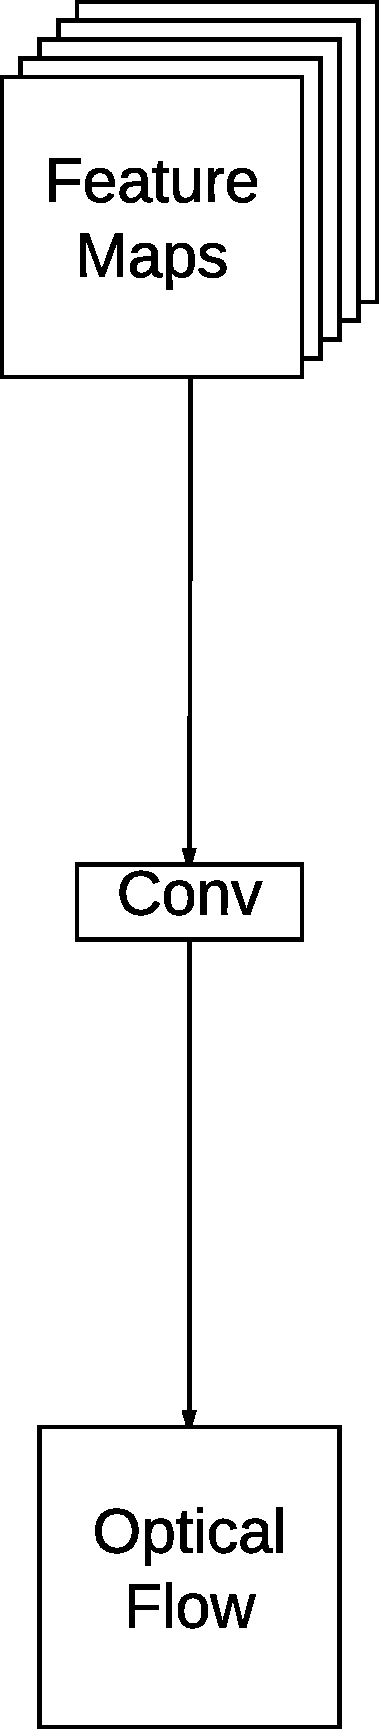
\includegraphics{Pic/PDF/NetworkStructure/Normal.pdf}}}
  &
  \resizebox{0.21\textwidth}{!}{\rotatebox{0}{
  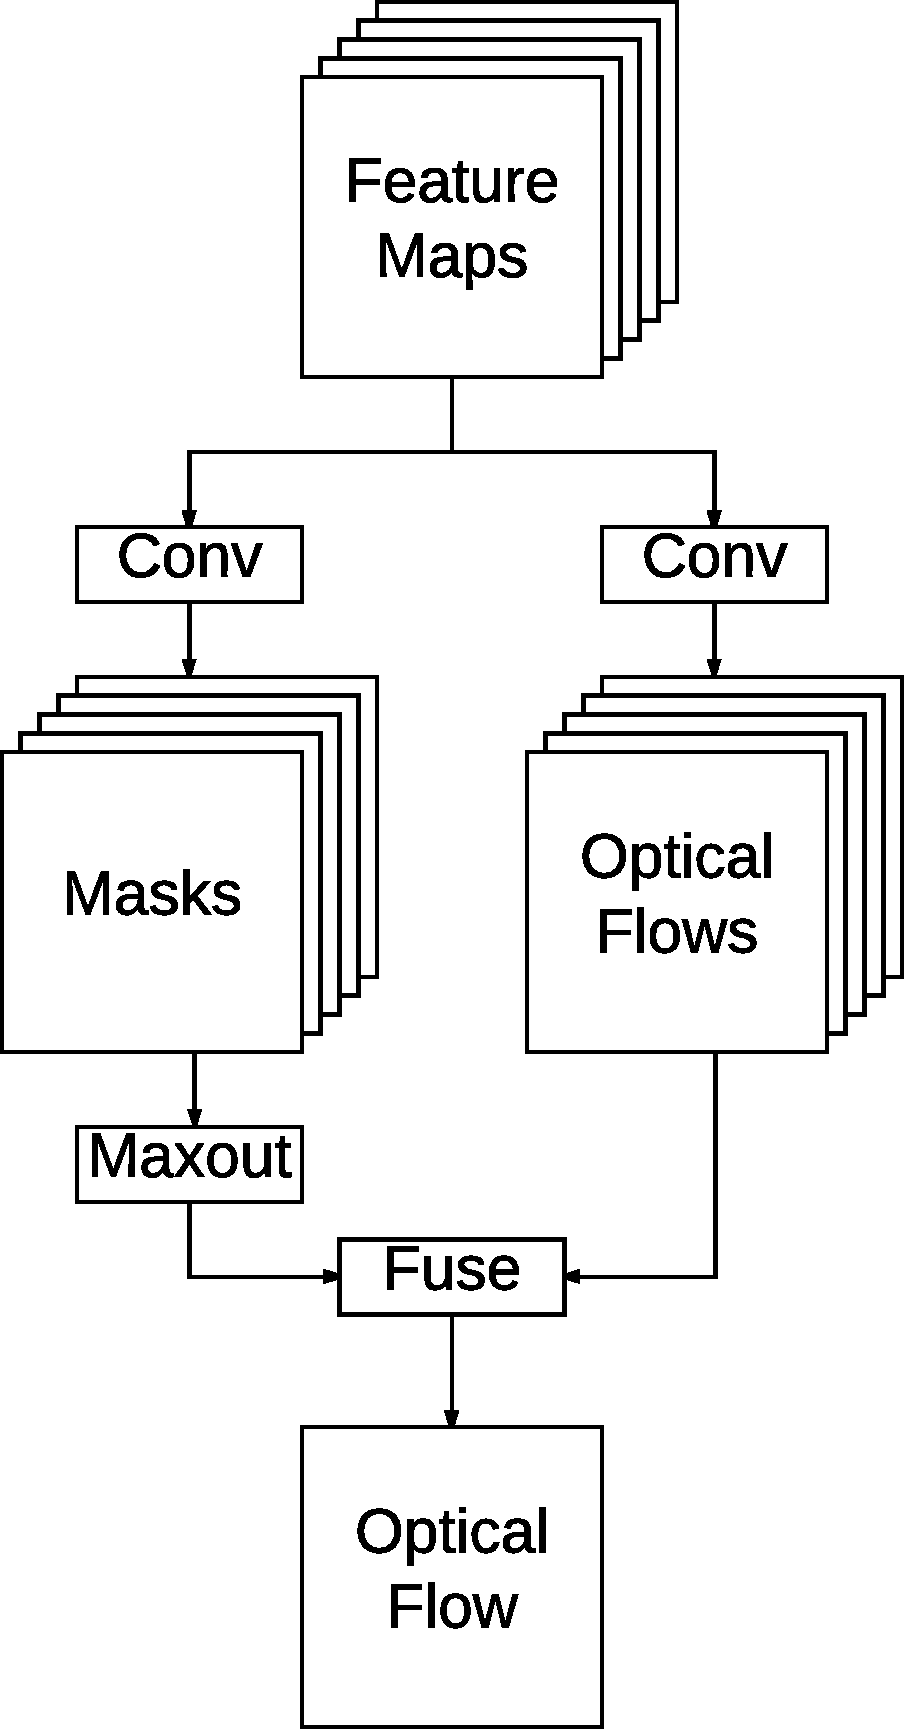
\includegraphics{Pic/PDF/NetworkStructure/MaskModule.pdf}}}
  \\
  a. Normal output & b. Soft-masks module 
  \\
\end{tabular}}
\caption{An illustration of the structure of the proposed soft-masks module compared with normal linear optical flow output.}
\label{fig: soft-masks module}
\end{figure} 

\subsection{Soft-masks module}
FlowNet~\cite{7410673} is the first work that uses deep convolutional neural network for flow estimation. The network architecture used by FlowNet is very similar to classical structure of auto-encoder, where optical flows are generated using deconvolution at each scale level of the image pyramid. To refine estimation of the flows, shortcuts are built to connect layers of corresponding level in encoder and decoder. Let's take a look at a single computation of convolution, and for simplicity, let's assume $f$ represents both horizontal and vertical components of an output flow. Given $X \in \mathbb{R}^{s\times s \times c}$, representing a volume feature vector in the input feature volume, inputted to output layer,  where $s$ is kernel size and $c$ is number of channels. FlowNet employs a linear activation to compute optical flow:

\begin{equation}
f = X^T W + b
\end{equation}

\begin{figure}[h]
\centerline{
\begin{tabular}{c}
  \resizebox{0.3\textwidth}{!}{\rotatebox{0}{
  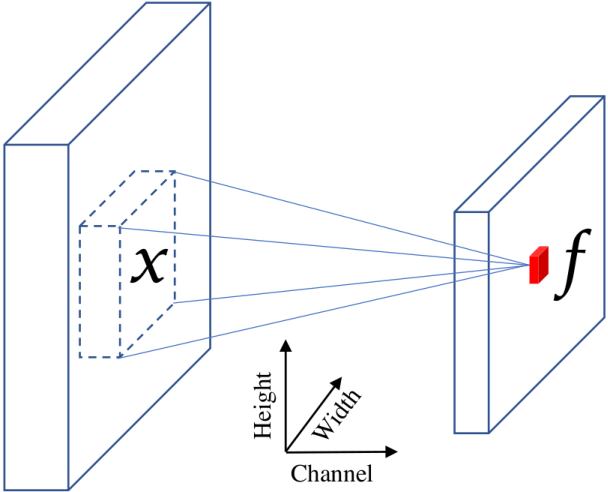
\includegraphics{Pic/PDF/conv_demo-crop.pdf}}}
  \\
\end{tabular}}
\caption{An illustration of annotation used in convolution.}
\label{fig: conv_layer}
\end{figure} 

Given actual optical flow field a nonlinear and piece-wise smooth representation of motions contained in images, using linear function to fit the flow field is less accurate. We introduce a soft-masks module in this paper. The proposed module can be used to replace the linear output of optical flow estimation. We will show that by using this module, we are able to separate optical flow field to multiple layers. Flow estimation in each layer is smooth and can be estimated using a quadratic function, which results in a more accurate and flexible optical flow estimation. 

An illustration of soft-masks module is shown in Figure~\ref{fig: soft-masks module}. The essential part of the soft-masks module is its dual-branch structure which contains mask branch and optical flow branch. The same input feature maps represented as a set of volume feature vectors, $X \in \mathbb{R}^{s\times s \times c}$ thus are imported to both branches. The most significant contribution of this work is to separate one optical flow field to multiple layers. For a separation of $k$ layers. $k$ masks will be generated in mask branch as illustrated in Figure~\ref{fig: soft-masks module}, which requires $k$ convolutional filters labeled as $\{W_n^m, b_n^m\}_{n=1}^k$ being used in mask branch. Correspondingly, the same number of filters are used in optical flow branch which are labeled as $\{W_n^f, b_n^f\}_{n=1}^k$. Then the mask and intermediate optical flow could be computed as following:

\begin{align}
\label{eqn: computation of masks and flows}
m_n =& X^T W_n^m + b_n^m &\! \text{for $n = 1\dots k$} \nonumber\\
f_n =& X^T W_n^f + b_n^f &\! \text{for $n = 1\dots k$}
\end{align}
Thus, give $k$ filters used in both branches, we will obtain $k$ corresponding pairs of mask and intermediate optical flow. Basically, by using $k$ filters in optical flow branch and generating $k$ intermediate optical flow, we assume each filter will work independently and being active only to a single type or a few types of object motions. Correspondingly, filters in mask branch are expected to have some behaviors that each of the generated masks which indeed are active maps should be high active for certain types of motions in some region and low active for other types of motions in other regions. This inspires us to use a maxout operation to extract mask entries with maximal activation along channel axis. So, after maxout operation, for each mask $m_n, n=1\dots k$, all entries will be zero-out except entries whose activation value are maximal in the some region among all masks. We denote masks after maxout as $\{m_n'\}_{n=1}^k$. Thus, there is no intersection among masks in $\{m_n'\}_{n=1}^k$ and the union of all $m_n', n=1\dots k$ has activation in full region. The maxout can be represented as following:

\begin{equation}
\label{eqn: maxout}
m_n'=
\begin{cases}
m_n, & \text{if}\ m_n = \max\limits_{p=1\dots k}(m_p) \\
0, & \text{otherwise}
\end{cases} \quad \text{for $n = 1\dots k$}
\end{equation}

It could be seen from Equation~\ref{eqn: maxout}, the masks after maxout are not converted to binary masks. This is the reason why the module is called soft-masks module. 

\begin{figure}[h]
\centerline{
\begin{tabular}{c}
  \resizebox{0.3\textwidth}{!}{\rotatebox{0}{
  
\includegraphics{Pic/PDF/PicHere.pdf}}}
  \\
\end{tabular}}
\caption{An illustration of how maxout is working for soft-masks module.}
\label{fig: maxout demo}
\end{figure} 

Masks after maxout operation are applied to corresponding intermediate optical flows by element-wise multiplication which is shown in below:

\begin{figure*}[th]
\centerline{
\begin{tabular}{c}
  \resizebox{0.92\textwidth}{!}{\rotatebox{0}{
  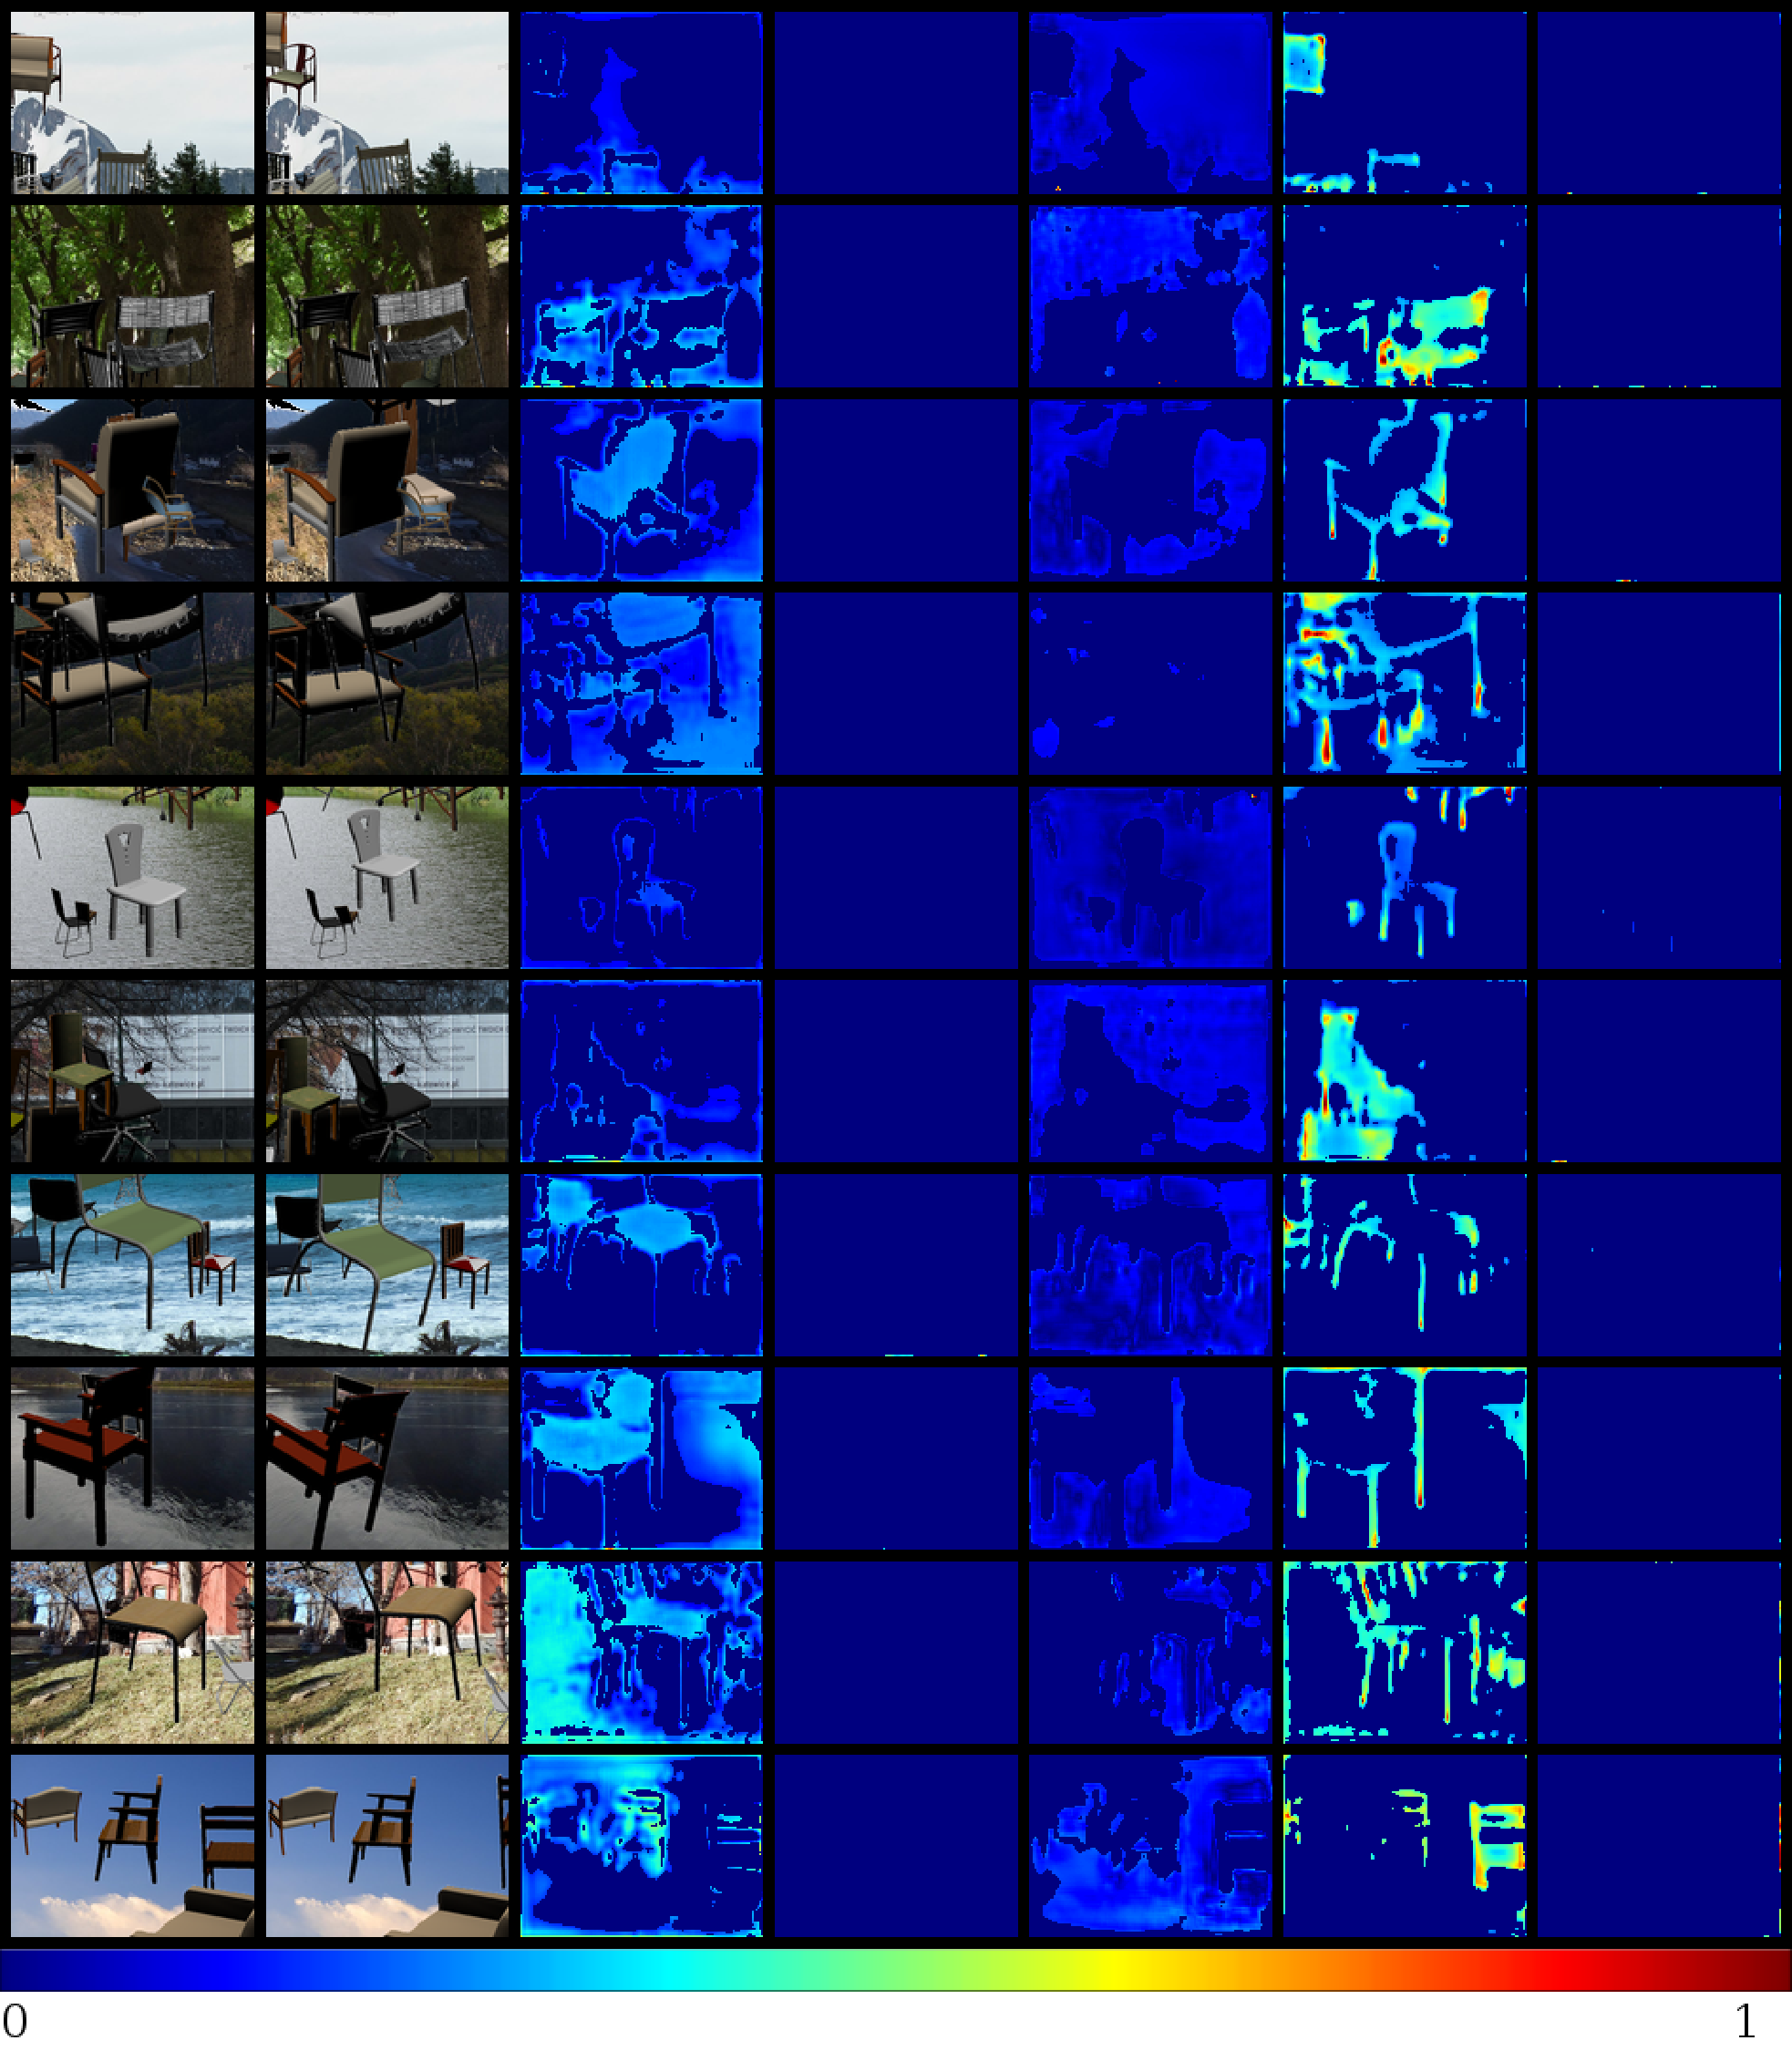
\includegraphics{Pic/PDF/Masks_demo.pdf}}}
  \\
\end{tabular}}
\caption{Examples of generated masks using the proposed soft-mask module. In this example, five masks are generated for each input image pair.Mask values are rearranged to ones between 0 and 1 for rendering.}
\label{fig: maxout demo}
\end{figure*} 

\begin{equation}
\label{eqn: maxout}
f_n'=
\begin{cases}
m_n' \times f_n, & \text{if}\ m_n' \neq 0 \\
0, & \text{otherwise}
\end{cases} \quad \text{for $n = 1\dots k$}
\end{equation}
Results of the above computation is a set of disjoint optical flow layers, each of which represent a certain type of motion. An illustration of how soft-masks module works is show in Figure~\ref{fig: maxout demo} and results of generated masks are show in Figure~\



\subsection{Quadratic fitting of optical flows}
Objects move in different ways in images, which results in different types of motion. The underlying optical flows thus are non-linear and locally piece-wise smooth. 

There are two consequences of using soft-masks module that could make estimation of the optical flow easier. The first advantage of using soft-masks module originate from usage of maxout in generating masks. By keeping only the maximal value among all masks, the optical flows are forced to be separated to multiple disjoint layers. Theoretically proofing maxout will result in a precise cut along motion boundary is challenging and is still under our investigation. However, qualitative results shown in Figure~\ref{fig: maxout demo} demonstrate that soft-masks module enable resulting masks to separate flow field to pieces according to detected motion types. In addition, the masks detects boundary of each piece as well, which enables estimation of optical flows on boundary more accurate.  Secondly, The estimation of optical flows using the proposed soft-masks module is quadratic in terms of feature maps $X$ inputed to the module.

To show this, given the computation of masks and intermediate optical flows shown in Equation~\ref{eqn: computation of masks and flows}, the computation of non-zero $f_n'$ could be written as:

\begin{align}
f_n' & = m_n' \times f_n \nonumber\\
	 & = (X^T W_n^m + b_n^m) \times (X^T W_n^f + b_n^f) \nonumber\\
	 & = W_n^m X X^T W_n^f + X^T(b_n^f W_n^m + b_n^m W_n^f) + b_n^m b_n^f
\end{align}
As shown in above equation, the representation of $f_n'$ is quadratic in terms of variable $X$.

To better illustrate the difference of using soft-masks module with respect to linear output, a 1D example is show in Figure~\ref{fig: quadratic demo}. In the example, function values are smooth in three separate ranges. The improvement of fitting data using piecewise quadratic function over linear function could be seen from this example. 

\begin{figure}[h]
\centerline{
\begin{tabular}{ccc}
  \resizebox{0.15\textwidth}{!}{\rotatebox{0}{
  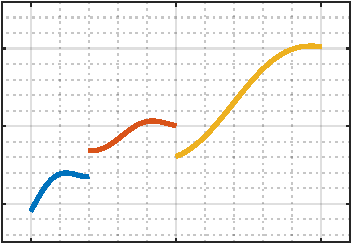
\includegraphics{Pic/PDF/QuadraticFuncDemo/FitDemo_1-crop.pdf}}}
  &
  \resizebox{0.15\textwidth}{!}{\rotatebox{0}{
  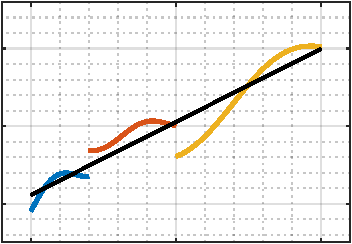
\includegraphics{Pic/PDF/QuadraticFuncDemo/FitDemo_2-crop.pdf}}}
  &
  \resizebox{0.15\textwidth}{!}{\rotatebox{0}{
  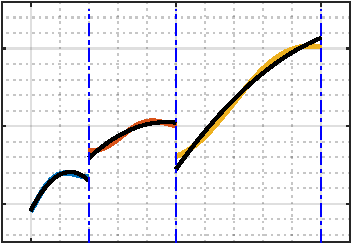
\includegraphics{Pic/PDF/QuadraticFuncDemo/FitDemo_3-crop.pdf}}}
  \\
  A & B & C
  \\
\end{tabular}}
\caption{A: Given data. B: Fitting using linear function. C: Fitting using piece-wise quadratic function.}
\label{fig: quadratic demo}
\end{figure} 

\subsection{Regularization for Unsupervised Training}
Training an unsupervised neural network for optical flow estimation is available by using network similar to FlowNet as a base optical flow inferring network followed by a spatial transform network (STN)~\cite{jaderberg2015spatial}. Existing works such as: DSTFlow~\cite{ren2017unsupervised}, USCNN~\cite{ahmadi2016unsupervised}, and back-to-basic unsupervised FlowNet (bb-FlowNet)~\cite{DBLP:journals/corr/YuHD16} all follow the same framework and train  their train neural networks unsupervisely to minimize an objective defined in Equation~\ref{eqn: flow objective}.  To show the proposed soft-masks module can improve flow estimation under the same framework, we add the soft-masks module to FlowNet and use it as a base optical flow inferring network in unsupervised training framework.

Smoothness restriction which is used by all above mentioned unsupervised approaches plays a significant role in regularizing the local consistancy of optical flows.  We follow the traditional regularization term used to constraint deformation field~\cite{rohlfing2003volume}\cite{ashburner1999nonlinear} and define the regularization term used in Equation~\ref{eqn: flow objective} as following:

\begin{align*}
\varphi(\bold{u}, \bold{v}) = & \sum ((\frac{\partial^2\bold{u}}{\partial \bold{x}^2})^2+(\frac{\partial^2\bold{u}}{\partial \bold{y}^2})^2+2(\frac{\partial^2\bold{u}}{\partial \bold{x} \partial \bold{y}})^2) + \\ 
& \sum ((\frac{\partial^2\bold{v}}{\partial \bold{x}^2})^2+(\frac{\partial^2\bold{v}}{\partial \bold{y}^2})^2+2(\frac{\partial^2\bold{v}}{\partial \bold{x} \partial \bold{y}})^2)
\end{align*}


\section{Empirical Evaluation}
\label{sec: evaluation}
\subsection{Benchmark}
We evaluate our performance on three standard optical flow benchmarks: Flying Chairs~\cite{7410673},  Sintel~\cite{Butler:ECCV:2012}, and KITTI~\cite{geiger2012we}. We compare the performance of the proposed approach to both supervised methods such as: FlowNet(S/C)~\cite{7410673}, SPyNet~\cite{Ranjan_2017_CVPR} and DeepFlow~\cite{weinzaepfel2013deepflow}, EpicFlow~\cite{revaud2015epicflow} and  unsupervised methods including: DSTFlow~\cite{ren2017unsupervised}, USCNN~\cite{ahmadi2016unsupervised}, and back-to-basic unsupervised FlowNet (bb-FlowNet)~\cite{DBLP:journals/corr/YuHD16}. 

Recently, FlowNet 2.0, a follow-up work of FlowNet, achieves state of the art results on most datasets. The architecture of FlowNet 2.0~\cite{Ilg_2017_CVPR} resembles several FlowNets and contains cascade training of the FlowNets in different phases. Since the emphasis of this paper is to show soft-masks module can boost performance of a single network, we do not include FlowNet 2.0 in our evaluation. 

\subsection{Proposed Network Structure}
The goal of this paper is not to show a brand new design of a network and superior performance could be obtained using the network, instead, we are going to show performance improvement could be obtained by replacing normal optical flow output layer with soft-masks module. Based on this intention, we choose FlowNetS and FlowNetC as our base networks and replace their optical flow output layers with soft-masks module. Since we highlight the layered flow estimation (LOFE) in this paper, we term the resulting networks modified from FlowNet as FlowNetS+LOFE and FlowNetC+LOFE. 

One thing worth noticing is that although we chosen FlowNet to work on in our work, but since soft-masks module basically works as an add-on to a network, it can be used on wider selections of networks and vision tasks such as image segmentation~\cite{long2015fully}\cite{noh2015learning}, depth estimation in range images~\cite{eigen2014depth}\cite{eigen2015predicting}, etc..

\subsection{Training Details}
Both supervised and unsupervised networks are trained using Adam~\cite{kingma2014adam} optimization with $\beta_1=0.9$ and $\beta_2=0.999$. We use a small batch size of 8 across all dataset with 3000 iterations per epoch. The initial learning rate is set to be $1e-3$ and decrease to half every 60 epochs until the network converge. All experiments are finished on a single Nvidia 1080 GPU.

Various types of data augmentation are used during training. We apply rotation at random within $[\ang{-15}, \ang{15}]$. A random translation within $[-50, 50]$ pixels are applied to both horizontal and vertical directions. In addition, following~\cite{Ranjan_2017_CVPR} we include additive white Gaussian noise sampled uniformly from $\mathcal{N}(0, 0.1)$. We also apply color jitter with additive brightness, contrast and saturation samlped from a Gaussian, $\mathcal{N}(0, 0.4)$. All data augmentation are done using GPU during training.

\subsection{Results}
Evaluations are done with compared methods in two groups according to whether the training of the methods is unsupervised or not. Table~\ref{tab: results supervised} show the endpoint error (EPE) of the proposed network and several well known methods. Except EpicFlow and DeepFlow, all other methods in this table are trained in a supervised manner. Furthermore, we compare results of unsupervised method in Table~\ref{tab: results unsupervised}.

Note that in papers of FlowNet~\cite{Ilg_2017_CVPR} and SPyNet~\cite{Ranjan_2017_CVPR}, results are reported for fine-tuned network as well. Here we are not interested in the fine tuned results. Because we think fine tuning is tricky, the procedure of fine tuning may not be consistent among compared methods. Thus results using fine tuning can vary lot.   
\newline
\newline
\noindent \textbf{Supervised methods.} For FlowNetS+LOFE and FlowNetC+LOFE tested in this group, we use $k=10$ for both models. As can be seen from Table~\ref{tab: results supervised}, FlowNetS+LOFE and FlowNetC+LOFE achieve the best performance on all tests except on training set of Sintel Clean. Basically, the performance of FlowNetS and FlowNetC are both boosted by simply replace optical flow output layer with soft-masks module. Comparison of computation time shows that time increment due to replacement of soft-masks module is in an acceptable range. 
\newline
\newline
\noindent \textbf{Unsupervised methods.} Training optical flow estimation networks unsupervisely is straight forward by using objective shown in Equation~\ref{eqn: flow objective}. The tricky part is to decide the weight coefficient $\lambda$ in the equation. To choose an appropriate $\lambda$, we did a binary search for the best value in a range of $[0, 10]$. We stop such search when the improvement is small. For results of compared methods, the proposed networks achieve the best performance except for KITTI dataset. 

\begin{table*}[]
\centering
\caption{Average end point errors (EPE) of the proposed networks compared to several existing methods. EpicFlow and DeepFlow are traditional methods which do not use neural networks. All other methods in the table are trained supervisely. Bold font indicates the most accurate results among the network based methods.}
\label{tab: results supervised}
\begin{tabular}{lcccccccc}
\hline
\hline
\multicolumn{1}{c}{Method} & Flying Chairs & \multicolumn{2}{c}{Sintel Clean} & \multicolumn{2}{c}{Sintel Final} & \multicolumn{2}{c}{KITTI} & Time (s) \\
                           & Test          & Train           & Test           & Train           & Test           & Train            & Test   &          \\ \hline
EpicFlow                   & 2.94          & 2.40            & 4.12           & 3.7             & 6.29           & 3.47             & 3.8    & 16       \\
DeepFlow                   & 3.53          & 3.31            & 5.38           & 4.56            & 7.21           & 4.58             & 5.8    & 17       \\ \hline
FlowNetS                   & 2.71          & 4.50            & 7.42           & 5.45            & 8.43           & 8.26             & -      & 0.12     \\
FlowNetC                   & 2.19          & 4.31            & 7.28           & 5.87            & 8.81           & 9.35             & -      & 0.23     \\
SPyNet                     & 2.63          & \textbf{4.23}   & \textbf{6.82}           & 5.67            & 8.49           & 9.12             & -      & 0.11     \\
FlowNetS+LOFE              & 2.53          & 4.35            & 7.11           & \textbf{5.32}   & \textbf{8.25}  & \textbf{8.03}    & -      & 0.17     \\
FlowNetC+LOFE              & \textbf{2.08} & \textbf{4.23}            & 7.01  & 5.51            & 8.51           & 9.14             & -      & 0.30     \\ \hline
\end{tabular}
\end{table*}

\begin{table*}[]
\centering
\caption{EPE errors of methods that are trained unsupervisely. Results of compared methods are directly from corresponding paper.}
\label{tab: results unsupervised}
\begin{tabular}{lccccccc}
\hline
\hline
\multicolumn{1}{c}{Method} & Flying Chairs & \multicolumn{2}{c}{Sintel Clean} & \multicolumn{2}{c}{Sintel Final} & \multicolumn{2}{c}{KITTI}      \\
                           &               & Train           & Test           & Train          & Test            & Train          & Test          \\ \hline
DSTFlow                    & 5.11          & 6.93            & 10.40          & 7.82           & 11.11           & \textbf{10.43} & -             \\
USCNN                      & -             & -               & -              & 8.88           & -               & -              & -             \\
BB-FlowNet                 & 5.36          & -               & -              & -              & -               & 11.32          & \textbf{9.93} \\
FlowNetS+LOFE              & \textbf{4.81} & \textbf{6.56}   & 10.10          & \textbf{7.62}  & 10.98           & 10.78          & 10.82         \\
FlowNetC+LOFE              & 4.92          & 6.78            & \textbf{9.98}  & 7.77           & \textbf{10.19}  & 11.01          & 11.25         \\ \hline
\end{tabular}
\end{table*}

\subsection{Evaluation of Soft-masks Module}
Since we replaced simple linear output layer in FlowNet(S/C) with a relatively more complicated soft-masks module, one obvious question about our result is whether we obtained them by using a model with more coefficients rather than by the way of how soft-masks module works. Therefore, to better investigate the mechanism of soft-masks module, we compared the FlowNetC+LOFE with another two networks in which we slightly changed the structures of the soft-masks module.

In the first network, given the proposed structure as FlowNetC+LOFE, we removed maxout operation from soft-masks module and keep all other configuration the same. We term the resulting network as FlowNetC+LOFE/no-maxout. In this case FlowNetC+LOFE-v1 will have exact the same number of coefficients as FlowNetC+LOFE. For the second network, we totally removed the mask branch from soft-masks module and leave the intermediate optical flow branch only. The second network is denoted as FlowNetC+LOFE-v2. For all three networks, $k=5$ is used for soft-masks module. We use original FlowNetC as a baseline in this comparison. In order to obtain an unbiased comparison result, we train and test each of these networks on Flying Chairs dataset five times. The average EPE and standard deviation is reported in Table~\ref{tab: flownet variants}.

\begin{table}[]
\centering
\caption{Comparison of the proposed FlowNet+LOFE and its two variants.}
\label{tab: flownet variants}
\begin{tabular}{lc}
\hline
\hline
                         & Flying Chairs \\ \hline
FlowNetC                 & 2.19 $\pm$ 0.021            \\
FlowNetC+LOFE            & 2.08 $\pm$ 0.018            \\
FlowNetC+LOFE/no-maxout  & 2.16 $\pm$ 0.021            \\
FlowNetC+LOFE/no-masks   & 2.22 $\pm$ 0.021            \\
\hline
\end{tabular}
\end{table}

As can be seen from Table~\ref{tab: flownet variants}, the proposed FlowNet+LOFE over-performed its two variants. This comparison leads to two conclusions. First, the better performance obtained by adding soft-masks module to FlowNet is not because a larger model being used. Since the no-maxout version of the proposed network indeed has the identical structure as the proposed network. It also means that maxout operation make optical flow estimation an easier task by separating optical flows to different layers. Second, it can be seen from the table,  performance of the no-maxout version is slightly better than that of the no-masks version. one explanation is that the model of no-maxout version is bigger than the model of no-masks version. However, model size is not a determining factor causing the difference of performance. Because, FlowNet, the smallest model in this comparison, achieved a better performance than no-masks version of model. We think the true reason leading to this result is a fact that the no-maxout version of model actually is using a quadratic function to fit optical flows rather than a linear function used by no-masks version. 

\begin{figure}[th]
\centerline{
\begin{tabular}{c}
  \resizebox{0.48\textwidth}{!}{\rotatebox{0}{
  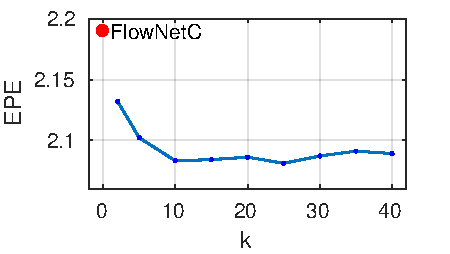
\includegraphics{Pic/PDF/k/K_Demo.pdf}}}
  \\
\end{tabular}}
\caption{EPE as a function of $k$, the number of layers used in soft-masks module.}
\label{fig: evaluation k}
\end{figure} 

We investigate the relationship between $k$ the number of mask and flow layers used in soft-masks module and network performance in terms of EPE. Experiments are done on Flying Chairs dataset. We start with a soft-masks module of $k=2$, then set $k=5\mathrm{x}, \mathrm{x}=1, \dots, 8$ for later experiments. It is easy to see from Figure~\ref{fig: evaluation k}, there is an immediate benefit of using soft-masks module with respect to FlowNetC, where even $k=2$ will efficiently boost the performance. On Flying Chairs dataset the curve in Figure~\ref{fig: evaluation k} quickly converge after $k=10$ and raise a bit when $k>25$. We think this is due to a slight overfitting when separating optical flow to too many layers. 



\section{Conclusion}
In summary, we have described a new way of optical flow estimation by combining traditional layered flow representation with deep learning method. rather than pre-segmenting image to layers, the proposed approach automatically learn layered representation of optical flow using the proposed soft-masks module. Soft-masks module offer a benefit of splitting flow to layers in which the computation of the flow is quadratic in terms of input feature. In evaluation, we use FlowNet as our base net to add the soft-masks module. The resulting networks are tested on three well known benchmark with both supervised and unsupervised flow estimation tasks. Empirical results show that the proposed network achieve better results with respect to the original FlowNet. 


{\small
\bibliographystyle{ieee}
\bibliography{mybib}
}

\end{document}
